% Typografie a publikování
% 3. projekt
% Juraj Holub
% xholub40@stud.fit.vutbr.cz

\documentclass[a4paper, 11pt]{article}
\usepackage[utf8]{inputenc}
\usepackage[czech]{babel}
\usepackage[left=2cm,top=3cm,text={17cm,24cm}]{geometry}
\usepackage[IL2]{fontenc}
\usepackage[hyphens,spaces,obeyspaces]{url}
\usepackage{hyperref}
\usepackage[czech]{babel}
\usepackage{times}
\usepackage{dsfont}
\usepackage{multirow}
\usepackage{amsmath, amsthm, amsfonts, amssymb}
\usepackage[linesnumbered,noline,boxed,commentsnumbered,ruled,longend]{algorithm2e}
\SetNlSty{}{}{:} 
\usepackage{graphicx}
\usepackage{float}
\usepackage{lscape}
\usepackage{tikz}
\usepackage{lipsum}
\usepackage{tabularx,booktabs}
\usepackage{setspace}
\usepackage{longtable}
\usepackage{threeparttable}

\newcolumntype{Y}{>{\centering\arraybackslash}X}

\author{Juraj Holub}
\date{}

\begin{document}


\begin{titlepage}
\begin{center}
	\Huge
	\textsc{\Huge{Vysoké učení technické v~Brně} \\
	\huge{ Fakulta informačních technologií}} \\
	\vspace{\stretch{0.382}}
	\LARGE{Formální jazyky a překladače} \\
	\Huge{Projektová dokumentácia} \\
	\Large{\today}
	\vspace{\stretch{0.618}}
	\setlength{\parindent}{0.3em}

	{\Large Tým 008, varianta II} \\
	
\begin{table}[H]
	\Large
	\centering
	\begin{tabular}{llc}
		\textbf{Člen}        & \textbf{Login} & \textbf{Rozdelenie bodov} \\
		Juraj Holub (vedúci) & \texttt{xholub40}       & 33\%                      \\
		Matej Parobek        & \texttt{xparob00}       & 33\%                      \\
		Samuel Krempský      & \texttt{xkremp02}      & 33\%                      \\
		Vitalina Koloda      & \texttt{xkolod02}       & 0\%                      
	\end{tabular}
\end{table}
		
\end{center}
\end{titlepage}

{\hypersetup{hidelinks}\tableofcontents}
\newpage

\section{Rozdelenie práce}

Prácu na projekte sme rozdelili následovne:
\begin{itemize}
	\item{\textbf{Lexikálnu analýzu} vytvoril Samuel Krempský (\texttt{xkremp02}).}
	\item{\textbf{Syntaktickú analýzu zhora nadol} vytvoril Matej Parobek (\texttt{xparob00}).}
	\item{\textbf{Precedenčnú syntaktickú analýzu} vytvoril Juraj Holub (\texttt{xholub40}).}
	\item{\textbf{Tabuľku symbolov} vytvoril Juraj Holub (\texttt{xholub40}).}
	\item{\textbf{Generátor výstupneho kódu} vytvoril Juraj Holub (\texttt{xholub40}) a Matej Parobek (\texttt{xparob00}).}
	\item{\textbf{Sémantickú analýzu} aplikovanú pri syntaktickej analýze zhora nadol vytvoril Matej Parobek (\texttt{xparob00}) a pre precedenčnú analýzu Juraj Holub (\texttt{xholub40}).}
\end{itemize}
\section{Lexikálna analýza}
Hlavnými funkciami lexikálnej analýzy sú \texttt{get\_token()} a \texttt{ret\_token()}. Funkcia \texttt{get\_token()} je implementovaná ako konečný automat, ktorý je implementovaný pomocou podmienok a konštánt. Ak sa konečný automat dostane do konečného stavu tak vracia tzv. token. Niekedy však táto funkcia musí načítať aj jeden znak z ďalšieho tokenu, aby vedela,že je v konečnom stave.Tento znak je predávaný globálnou premennou \texttt{nextchar}. 
%%probably will be deleted

%%Token reprezentuje štruktúra majúca dva prvky \texttt{int type}, kde predávame typ daného tokenu pomocou konštánt a \texttt{string\_t attribute}, čo je premenná dátového typu \texttt{string\_t} pre prácu s dynamickými reťazcami, kde predávame názov premennej, alebo text dátového typu string v jazyku IFJ18.

Funkcia \texttt{ret\_token()} vracia token z parseru scanneru. Potom čo je funkcia \texttt{get\_token()} spustená, tak pri ďalšom volaní je vrátený predošlý token. Táto funkcia je volaná parserom a môže požiadať až o dve predošlé tokeny, takže scanner musí mať stále uložené dva predošlé tokeny.

Diagram konečného automatu, který specifikuje lexikální analyzátor \ref{fsm}.

\begin{figure*}[!]
	\centering
	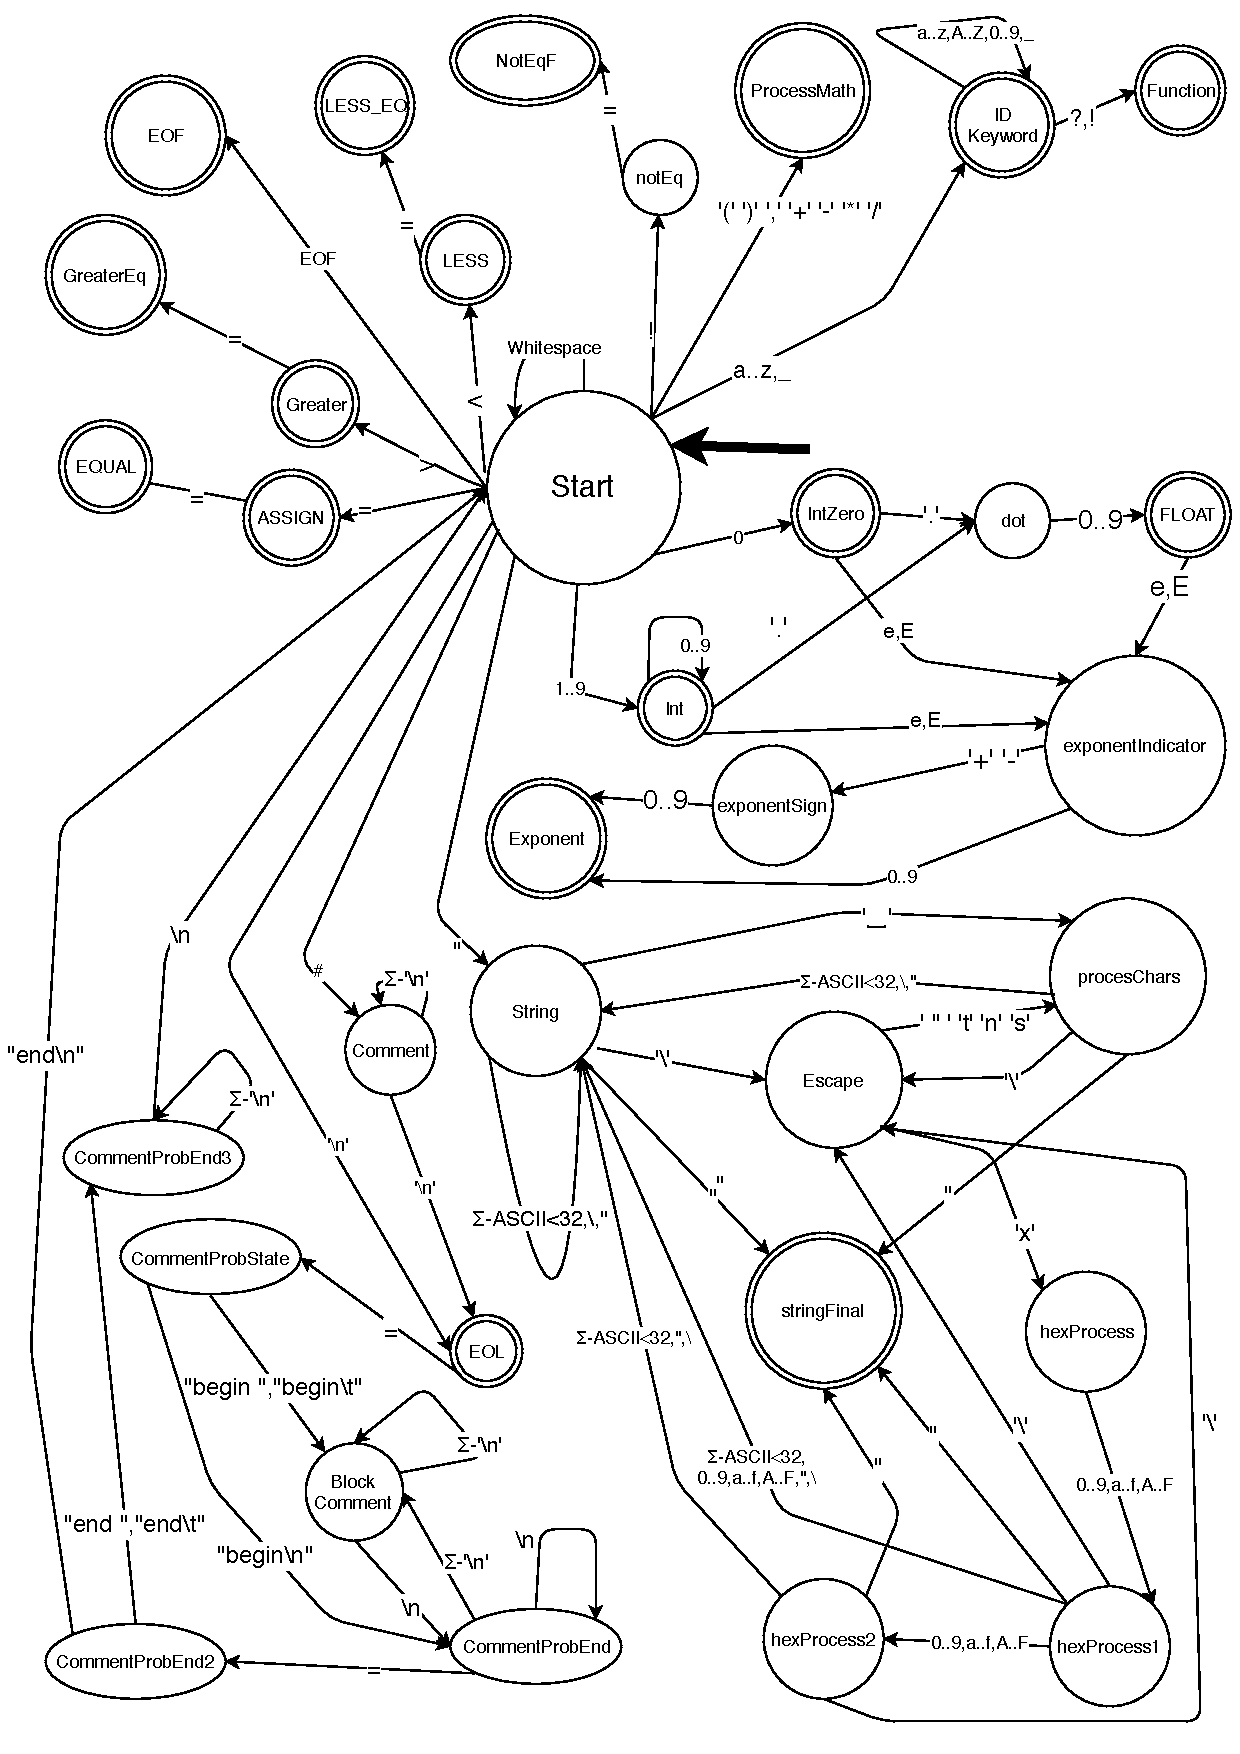
\includegraphics[width=\linewidth,height=8in]{fsm_scanner.pdf}\\[1pt]
	\caption{Diagram konečného automatu, který specifikuje lexikální analyzátor.}
	\label{fsm}
\end{figure*}

\newpage
{\Large{Legenda:}} 

\begin{itemize}
\item $\sum = \{ASCII\}$
\item EOL - vracia token konca riadku (ukončenia príkazu)
\item EOF - vracia token typu EOF (koniec zdrojového kódu)
\item ProcessMath - stav v ktorom sa pomocou pomocnej funkcie naďalej rozhoduje o aký typ tokenu sa jedná
\item NotEqF - vracia token nerovnosti 
\item LESS - vracia token ako relačný operátor menšie ako
\item LESS\_EQ - vracia token ako relačný operátor rovnosti
\item Greater - vracia token ako relačný operátor väčšie
\item GreaterEq - vracia token ako relačný operátor väčšie rovná sa
\item ASSIGN - vracia token priradenia
\item EQUAL - vracia token ako relačný operátor rovná sa
\item ID Keyword - stav v ktorom sa vyhodnocuje, či je daný reťazec znakov kľúčové slovo alebo identifikátor
\item Function - vracia sa token funkcie
\item IntZero - vracia token celého čísla nula
\item Int - vracia token celého čísla 
\item FLOAT - vracia token desatinného čísla
\item Exponent - vracia token čísla s exponentom
\item stringFinal - vracia token reťazca znakov

\end{itemize}
\newpage

\section{Syntaktická analýza zhora nadol}
Tabuľka \ref{ll_gram} popisuje LL gramatiku použitú pre syntaktickú analýzu zhora nadol. Tabuľka \ref{ll_tab} popisuje LL tabuľku pre danú LL gramatiku.

\begin{table*}[ht]
\begin{longtable}[l]{l l c l}
		1: & \textless program\textgreater & $\rightarrow$ & EOF \\
		2: & \textless program\textgreater & $\rightarrow$ & \textless program\textunderscore list\textgreater  EOF \\
		3: & \textless program\textunderscore list\textgreater & $\rightarrow$ & \textless function\textunderscore def\textgreater  \textless program\textunderscore list\textgreater \\
		4: & \textless program\textunderscore list\textgreater & $\rightarrow$ & \textless statement\textgreater  \textless program\textunderscore list\textgreater \\
		5: & \textless function\textunderscore def\textgreater & $\rightarrow$ & def ID/FUN ( \textless params\textgreater \\
		6: & \textless params\textgreater & $\rightarrow$ &  ) EOL \textless function\textunderscore body\textgreater \\
		7: & \textless params\textgreater & $\rightarrow$ & ID \textless param\textunderscore list\textgreater \\
		8: & \textless param\textunderscore list\textgreater & $\rightarrow$ &  ) EOL \textless function\textunderscore body\textgreater \\
		9: & \textless param\textunderscore list\textgreater & $\rightarrow$ &  , ID \textless param\textunderscore list\textgreater \\
		10: & \textless function-body\textgreater & $\rightarrow$ & \textless statement\textgreater \textless fun\textunderscore body\textgreater \\
		11: & \textless function-body\textgreater & $\rightarrow$ & end EOL \\
		12: & \textless statement\textgreater & $\rightarrow$ & \textless if\textunderscore statement\textgreater \\
		13: & \textless statement\textgreater & $\rightarrow$ & \textless while\textunderscore statement\textgreater \\
		14: & \textless statement\textgreater & $\rightarrow$ & \textless assignment\textgreater  EOL \\
		15: & \textless if\textunderscore statement\textgreater & $\rightarrow$ &  if \textless expression\textgreater  then EOL \textless if\textunderscore body\textgreater \\
		16: & \textless if\textunderscore body\textgreater & $\rightarrow$ & \textless statement\textgreater \textless if\textunderscore body\textgreater \\
		17: & \textless if\textunderscore body\textgreater & $\rightarrow$ & else EOL \textless else\textunderscore body\textgreater \\
		18: & \textless else\textunderscore body\textgreater & $\rightarrow$ & \textless statement\textgreater \textless else\textunderscore body\textgreater \\
		19: & \textless else\textunderscore body\textgreater & $\rightarrow$ & end EOL \\
		20: & \textless while\textunderscore statement\textgreater & $\rightarrow$ & while \textless expression\textgreater  do EOL \textless while\textunderscore body\textgreater \\
		21: & \textless while\textunderscore body\textgreater & $\rightarrow$ & \textless statement\textgreater \textless while\textunderscore body\textgreater \\
		22: & \textless while\textunderscore body\textgreater & $\rightarrow$ & end EOL \\
		23: & \textless assignment\textgreater & $\rightarrow$ & ID = \textless function\textunderscore call\textgreater \\ 
		24: & \textless assignment\textgreater & $\rightarrow$ & ID = \textless expression\textgreater \\ 
		25: & \textless assignment\textgreater & $\rightarrow$ & \textless function\textunderscore call\textgreater \\ 
		26: & \textless assignment\textgreater & $\rightarrow$ & \textless expression\textgreater \\
		27: & \textless function\textunderscore call\textgreater & $\rightarrow$ & ID/FUN \textless call\textunderscore params\textgreater  EOL \\
		28: & \textless call\textunderscore params\textgreater & $\rightarrow$ & (\textless call\textunderscore param\textgreater ) \\
		29: & \textless call\textunderscore params\textgreater & $\rightarrow$ & \textless call\textunderscore param\textgreater \\
		30: & \textless call\textunderscore param\textgreater & $\rightarrow$ & $\varepsilon$ \\
		31: & \textless call\textunderscore param\textgreater & $\rightarrow$ & ID/CONST \textless call\textunderscore param\textunderscore list\textgreater \\
		32: & \textless call\textunderscore param\textunderscore list\textgreater & $\rightarrow$ & $\varepsilon$ \\
		33: & \textless call\textunderscore param\textunderscore list\textgreater & $\rightarrow$ & , ID/CONST \textless call\textunderscore param\textunderscore list\textgreater \\
\end{longtable}
\caption{LL gramatika.}
\label{ll_gram}
\end{table*}

\begin{table*}[ht]
\begin{threeparttable}
\centering
\resizebox{\linewidth}{!}{
\begin{tabular}{| l | c | c | c | c | c | c | c | c | c | c | c | c | c | c | c |}
		\hline
		 & \bf EOF & \bf EOL & \bf ID & \bf FN \tnote{a} & \bf def & \bf , & \bf end & \bf if & \bf else & \bf while & \bf = & \bf ( & \bf ) & \bf EXP \tnote{b} & \bf CONS \tnote{c} \\ \hline
		\bf \textless program\textgreater & 1 & 2 & 2 & 2 & 2 &   &   & 2 &   & 2 &   & 2 &   & 2 & 2 \\ \hline
		\bf \textless program\textunderscore list\textgreater &   & 4 & 4 & 4 & 3 &   &   & 4 &   & 4 &   & 4 &   & 4 & 4 \\ \hline
		\bf \textless function\textunderscore def\textgreater &   &   &   &   & 5  &   &   &   &   &   &   &   &   &   &   \\ \hline
		\bf \textless params\textgreater &   &   & 7 &   &   &   &   &   &   &   &   &   & 6 &   &   \\ \hline
		\bf \textless param\textunderscore list\textgreater &   &   &   &   &   & 9 &   &   &   &   &   & 8 &   &   &   \\ \hline
		\bf \textless function-body\textgreater &   &   & 10 & 10 &   &   & 11 & 10 &   & 10 &   & 10 &   & 10 &   \\ \hline
		\bf \textless statement\textgreater &   & 14 & 14 & 14 &   &   &   & 12 &   & 13  &   & 14 &   & 14 &   \\ \hline
		\bf \textless if\textunderscore statement\textgreater &   &   &   &   &   &   &   &   & 15 &   &   &   &   &   &   \\ \hline
		\bf \textless if\textunderscore body\textgreater &   &   & 16 & 16 &   &   &   & 16  & 17 &   & 16 &   & 16 & 16 & 16 \\ \hline
		\bf \textless else\textunderscore body\textgreater &   &   & 18 & 18 &   &   & 19 & 18 &   & 18 &   & 18 &   & 19 & 18 \\ \hline
		\bf \textless while\textunderscore statement\textgreater &   &   &   &   &   &   &   &   &   &   & 20 &  &   &   &   \\ \hline
		\bf \textless while\textunderscore body\textgreater &   &   & 21 & 21 &   &   & 22 & 21 &   & 21 &   & 21 &   & 21 & 21 \\ \hline
		\bf \textless assignment\textgreater &   & 26 & 23, 24, 25, 26 & 25 &   &   &   &   &   &   &   & 26 &   & 26 & 26 \\ \hline
		\bf \textless function\textunderscore call\textgreater &   &   & 27 & 27 &   &   &   &   &   &   &   &   &   &   &   \\ \hline
		\bf \textless call\textunderscore params\textgreater &   &   & 29 &   &   &   &   &   &   &   &   & 28 &   &   & 29 \\ \hline
		\bf \textless call\textunderscore param\textgreater &   & 30 & 31 &   &   &   &   &   &   &   &   &   & 30 &   & 31 \\ \hline
		\bf \textless call\textunderscore param\textunderscore list\textgreater &   & 32 &   &   &   &   & 33 &   &   &   &   &   & 32 &   &  \\ \hline
\end{tabular}
}
\begin{tablenotes}
	\footnotesize
	\item [a] \textbf{FN:} \underline{\textit{identifikátor obsahujúci nepovinný ! alebo ? na konci}}
	\item [b] \textbf{EXP:} \underline{\textit{not, -, +, *, /, ==, !=, \textless , \textless  =, \textgreater , \textgreater = }}
	\item [c] \textbf{CONS:} \underline{\textit{boolovská, celočíselná, desatinná a reťazcová konštanta}}
\end{tablenotes}
\end{threeparttable}
\caption{LL tabuľka.}
\label{ll_tab}
\end{table*}

\newpage
\section{Precedenčná syntaktická analýza}
Pre precedenčnú syntaktickú analýzu sme použili tabuľku \ref{prec_tab}. Symboly '$<$', '$>$', ' ' majú rovnaký význam ako značenie používané v predmete IFJ.
Legenda vstupných symbolov pre precedenčnú tabuľku \ref{prec_tab}:
\begin{itemize}
	\item{\textbf{NEG}: Operátor negácie boolovského výrazu (\texttt{\textbf{not}}) .}
	\item{\textbf{MINUS}: Operátor odčítania (\texttt{\textbf{-}}) typov float a integer.}
	\item{\textbf{PLUS}: Operátor sčítania alebo konkatenácia reťazcov (\texttt{\textbf{-}}).}
	\item{\textbf{MD}: Operátor násobenia alebo delenia (\texttt{\textbf{*}}, \texttt{\textbf{/}}).}
	\item{\textbf{EQ}: Relačný operátor (\texttt{\textbf{==}},\texttt{\textbf{!=}},\texttt{\textbf{<}},\texttt{\textbf{<=}},\texttt{\textbf{>}},\texttt{\textbf{>=}}).}
	\item{\textbf{ID}: Operand.}
	\item{\textbf{(}: Ľavá zátvorka vo výraze.}
	\item{\textbf{)}: Pravá zátvorka vo výraze.}
	\item{\textbf{\$}: Koniec výrazu (\texttt{\textbf{do}} , \texttt{\textbf{then}} , \texttt{\textbf{EOL}} , \texttt{\textbf{EOF}}) .}
\end{itemize}

\begin{table}[H]
	\centering
	\begin{tabularx}{\textwidth}{|c| *{9}{Y|}}%{|l|c|c|c|c|c|c|c|c|c|}
		\hline
		& \multicolumn{1}{c|}{\textbf{NEG}} & \multicolumn{1}{c|}{\textbf{MINUS}} & \multicolumn{1}{c|}{\textbf{PLUS}} & \multicolumn{1}{c|}{\textbf{MD}} & \multicolumn{1}{c|}{\textbf{EQ}} & \multicolumn{1}{c|}{\textbf{ID}} & \multicolumn{1}{c|}{\textbf{(}} & \multicolumn{1}{c|}{\textbf{)}} & \multicolumn{1}{c|}{\textbf{\$}} \\ \hline
		\textbf{NEG} & ' ' & ' ' & ' ' & ' ' & '\textless{}' & '\textless{}' & '\textless{}' & '\textgreater{}' & '\textgreater{}' \\ \hline
		\textbf{MINUS} & '\textgreater{}' & '\textgreater{}' & '\textgreater{}' & '\textless{}' & '\textgreater{}' & '\textless{}' & '\textless{}' & '\textgreater{}' & '\textgreater{}' \\ \hline
		\textbf{PLUS} & '\textgreater{}' & '\textgreater{}' & '\textgreater{}' & '\textless{}' & '\textgreater{}' & '\textless{}' & '\textless{}' & '\textgreater{}' & '\textgreater{}' \\ \hline
		\textbf{MD} & '\textgreater{}' & '\textgreater{}' & '\textgreater{}' & '\textgreater{}' & '\textgreater{}' & '\textless{}' & '\textless{}' & '\textgreater{}' & '\textgreater{}' \\ \hline
		\textbf{EQ} & '\textgreater{}' & '\textless{}' & '\textless{}' & '\textless{}' & '\textless{}' & '\textless{}' & \textbf{'\textless{}'} & \textbf{'\textgreater{}'} & \textbf{'\textgreater{}'} \\ \hline
		\textbf{ID} & '\textgreater{}' & '\textgreater{}' & '\textgreater{}' & '\textgreater{}' & '\textgreater{}' & ' ' & ' ' & '\textgreater{}' & '\textgreater{}' \\ \hline
		\textbf{(} & '\textless{}' & '\textless{}' & '\textless{}' & '\textless{}' & '\textless{}' & '\textless{}' & '\textless{}' & '=' & ' ' \\ \hline
		\textbf{)} & '\textgreater{}' & '\textgreater{}' & '\textgreater{}' & '\textgreater{}' & '\textgreater{}' & '\textgreater{}' & ' ' & '\textgreater{}' & '\textgreater{}' \\ \hline
		\textbf{\$} & '\textless{}' & '\textless{}' & '\textless{}' & '\textless{}' & '\textless{}' & '\textless{}' & '\textless{}' & '\textless{}' & ' ' \\ \hline
	\end{tabularx}
	\caption{Precedenčná tabuľka.}
	\label{prec_tab}
\end{table}

\section{Sémantická anylýza}
Semantické kontrolu sme vykonávali vždy po syntaktickej kontrole jedného pravidla LL gramatiky alebo precedenčnej tabuľky. Pre dané pravidlo v LL tabuľke alebo akciu v precedenčnej tabuľke sme vykonali príslušné sémantické kontroly a v prípadne úspechu sme vygenerovali príslušný kód v cieľovom jazyku IFJcode18.

\section{Generátor kódu}
Generovaný kód sme ukládali do listu, kde jedna položka listu predstavuje jednu inštrukciu v cieľovom jazyku IFJcode18. V liste sme aplikovali logické preusporiadanie vždy po ukončení vyhodnocovania aktuálneho rámca a to tak aby všetky premenné boli definované a inicializovane na hodnotu \texttt{nil} na začiatku daného rámca. Po ukončení všetkých analýz sme jedným priechodom vygenerovali celý list na štandartný výstup.
\section{Tabuľka symbolov}
Tabuľku symbolov sme implementovali ako \textbf{Tabuľku s rozptýlenými položkami} (\textbf{TRP}). Využili sme TRP s \textbf{explicitním} zreťazením synoným. TRP sme implementovali ako pole synoným o veľkosti 53 položiek. Veľkosť mapovacieho poľa sme zvolili ako prvočíslo a krok s veľkosťou jedna. Takúto veľkosť poľa synoným sme zvolili vzhľadom na jej výhodné chovanie, ktoré sme preberali v predmete IAL (nedochádza k vytváraniu zhlukov). Každá položka v mapovaciom poli obsahuje lineárny zoznam synoným. Keďže tabuľku využívame ako úložisko lexém programovacieho jazyka tak sme ako vyhľadávací kľúč použili názov identifikátoru premennej, ktorý musí byť unikátny. Pre vhodné mapovanie sme použili hashovaciu funkciu, ktorá poskytuje dobré výsledký pre reťazcové kľúče. Ako hash funkciu sme zvolili algoritmus \textbf{djb2}\footnote{Zdroj hash funkcie dbj2: 
	\urlstyle{rm}
	\url{http://www.cse.yorku.ca/~oz/hash.html}}
, ktorý má dobré výsledky práve pre reťazcové kľúče.
\section{Zhodnotenie}
Spolupráca v týme bola dostatočná. Komunikovali sme najviac elektronicky ale prebiehali aj pravidelné osobné stretnutia. Na začiatku sme si určili predbežné rozdelenie úloh, ktoré sa podľa potreby upravovalo. Taktiež sme si stanovili komunikačné kanály, možné termíny pre osobné stretnutia a \texttt{house style} zdrojového kódu. Na verzovanie sme použili verzovací systém \texttt{git}.


\end{document}
